\chapter{الشغل والطاقة والطاقة الكامنة}\label{ch:b1:work-and-energy}

يكفّ دراج عن الدوس في أعلى تلّة فيصل إلى الأسفل
بسرعة تتوقف على مقدار الهبوط لا على شكل الطريق. ويسقط
قافز بالحبل المطاطي ستين مترًا فيتوقف، لحظةً، عند الموضع
الذي يكون فيه شدّ الحبل قد أكل كل السرعة التي منحه إياها
السقوط. وتهتزّ ذرة هدروجين مرتبطة بذرة كلور في بئر
عمقها هو الطاقة التي يكلّفها تمزيق الجزيء. وفي كل
حالة يُتبادَل عدد واحد بين صور --- الحركة والارتفاع والاستطالة
والرابطة --- ولا يتغير مجموعه. ويبني هذا الفصل هذه
المحاسبة انطلاقًا من قانون نيوتن الثاني: \omterm{def:b1:work-and-energy:work}{الشغل} والاستطاعة، ومبرهنة
\omterm{thm:b1:work-and-energy:ke}{الطاقة الحركية}، والطاقات الكامنة للقوى التي تسمح بها،
\omterm{thm:b1:work-and-energy:em}{وانحفاظ الطاقة الميكانيكية} الذي يحوّل كثيرًا من مسائل الديناميك
إلى سطر واحد من الجبر، ويبيّن، عبر شكل \omterm{def:b1:work-and-energy:turning}{بئر الطاقة
الكامنة}، أيّ المواضع مستقرّ.

\begin{omfigure}
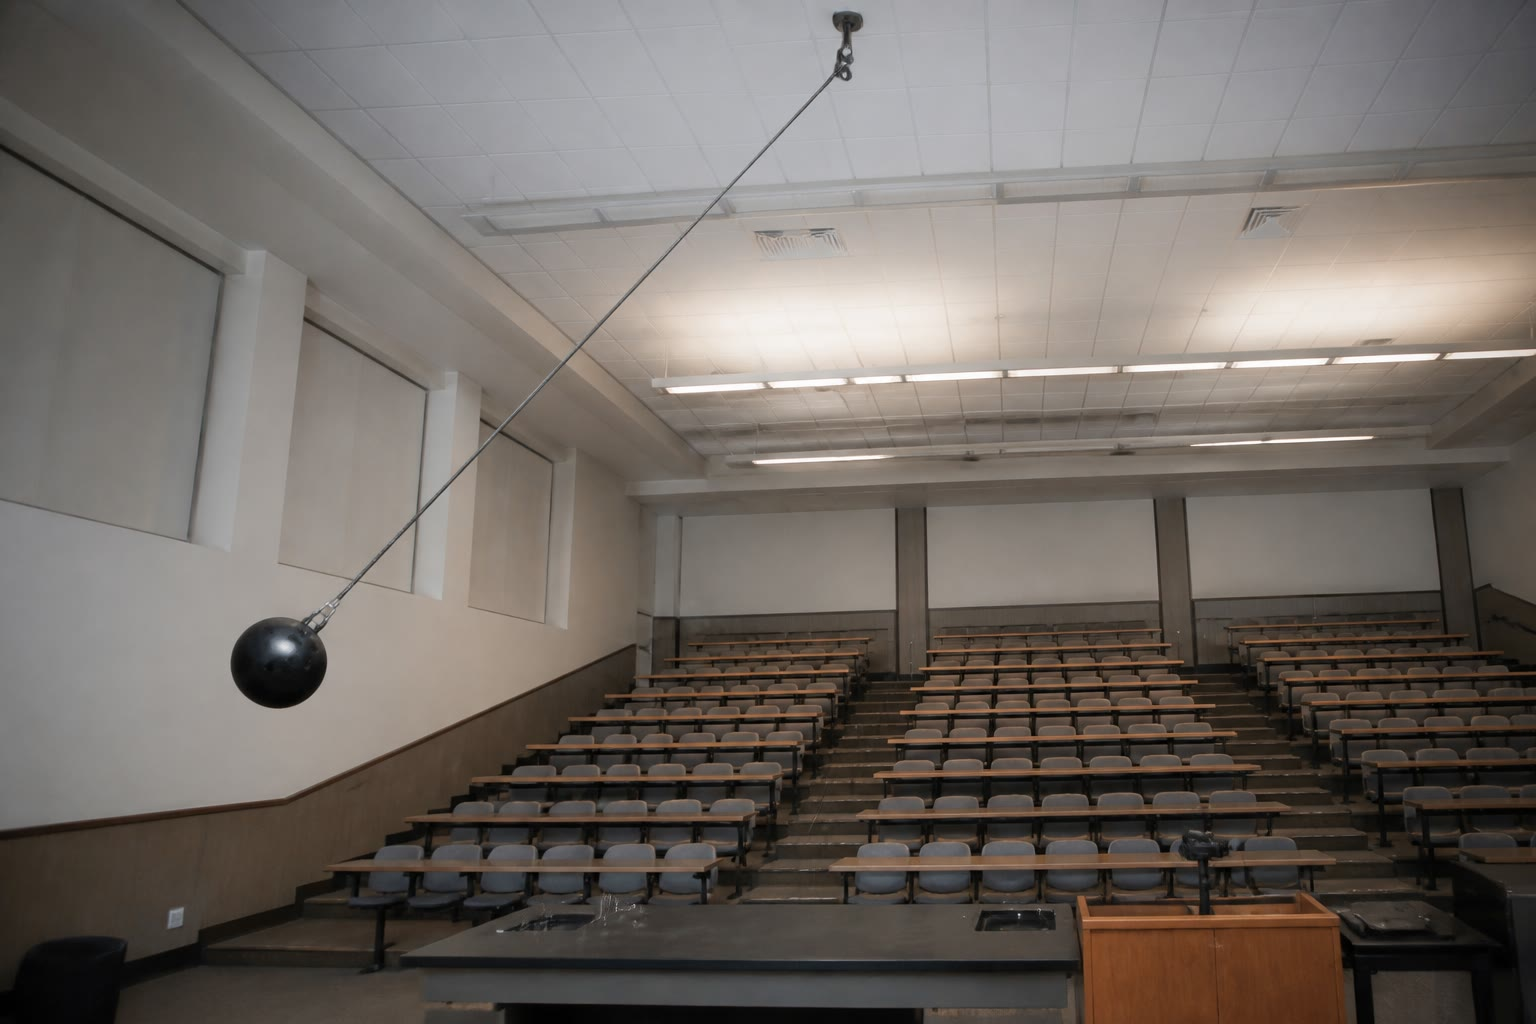
\includegraphics[width=0.58\linewidth]{images/book3/ai/b3-13-lecture-hall-pendulum.jpg}

{\small بندول المحاضرة: تُطلق كرة البولنغ من عند الأنف فتعود إلى الأنف ولا تتجاوزه --- \omterm{thm:b1:work-and-energy:em}{فالطاقة الميكانيكية} تنحفظ، ولا تُتجاوز قط.}
\end{omfigure}

\section{الاستطاعة والشغل}

\begin{definition}[استطاعة قوة وشغلها]\label{def:b1:work-and-energy:work}
\index{استطاعة قوة}\index{شغل}
إن \emph{استطاعة} قوة $\vect F$ مؤثرة في نقطة تتحرك بالسرعة
$\vect v$ هي
\[
\mathcal P = \vect F\cdot\vect v \qquad (\text{بالواط}),
\]
و\emph{شغلها} بين اللحظتين $t_1$ و $t_2$ (أي بين الموضعين $A$ و $B$)
هو الاستطاعة المتراكمة،
\[
W_{A\to B} = \int_{t_1}^{t_2}\vect F\cdot\vect v\,\dd t
= \int_A^B \vect F\cdot\dd\vect\ell \qquad (\text{بالجول}),
\]
أي مجموع \emph{الأشغال الأولية} $\delta W = \vect F\cdot\dd\vect\ell$
على امتداد الانتقالات الأولية $\dd\vect\ell = \vect v\,\dd t$ على
المسار. ويكون الشغل موجبًا إذا دفعت القوة في اتجاه الحركة
(فتكون \emph{محرّكة})، وسالبًا إذا عاكستها (فتكون \emph{مقاوِمة})، ومعدومًا إذا
كانت عمودية عليها.
\end{definition}

\begin{proposition}[أشغال تُصادَف]\label{prop:b1:work-and-energy:works}
\begin{itemize}
  \item قوة ثابتة: $W_{A\to B} = \vect F\cdot\vect{AB}$، أيًّا كان
        المسار. وللوزن: $W = mg(z_A - z_B)$، مع $z$ مقيسًا نحو الأعلى.
  \item نابض صلابته $k$، من الاستطالة $x_A$ إلى $x_B$:
        $W = \tfrac12 k(x_A^2 - x_B^2)$.
  \item ردّ الفعل العمودي لسطح ثابت، وشدّ خيط على جسم
        يتحرك عموديًّا عليه: $W = 0$ (فالقوة $\perp$ الانتقال).
  \item الاحتكاك الحركي والسحب: $W < 0$ دائمًا (لأن القوة تعاكس
        الحركة النسبية)، ويتوقف \omterm{def:b1:work-and-energy:work}{الشغل} على طول المسار.
\end{itemize}
\end{proposition}

\begin{proof}
من أجل $\vect F$ ثابتة: $\int\vect F\cdot\dd\vect\ell = \vect F\cdot\int\dd\vect\ell
= \vect F\cdot\vect{AB}$؛ ومع $\vect F = -mg\vect e_z$ يكون $\vect F\cdot\vect{AB}
= -mg(z_B - z_A)$. وللنابض: $\vect F\cdot\dd\vect\ell = -kx\,\dd x$، ومنه
$\int_{x_A}^{x_B}-kx\,\dd x = \tfrac12 k(x_A^2 - x_B^2)$. وللاحتكاك: $\vect T
= -\mu N\vect v/v$، ومنه $\vect T\cdot\vect v = -\mu Nv < 0$.
\end{proof}

\begin{omfigure}
\begin{tikzpicture}[font=\small, x=1cm, y=1cm]
  \draw[omDef, thick, domain=0:6, samples=60] plot (\x, {0.35*\x + 0.9*sin(deg(0.7*\x))});
  \fill (0,0) circle (1.4pt) node[below] {$A$};
  \fill (6,{2.1+0.9*sin(deg(4.2))}) circle (1.4pt) node[right] {$B$};
  % point at x=2.4: y = 0.84+0.9*sin(96.3deg)=0.84+0.894=1.734 ; slope 0.35+0.63cos(96.3)=0.35-0.069=0.28
  \coordinate (M) at (2.4,1.734);
  \fill[omThm] (M) circle (1.6pt); \node[above left] at (M) {$M$};
  \draw[-Stealth, omThm, very thick] (M) -- ++(1.1,0.31) node[right] {$\dd\vect\ell$};
  \draw[-Stealth, omProp, very thick] (M) -- ++(1.4,-0.9) node[below right] {$\vect F$};
  \draw ($(M)+(0.55,0.15)$) arc (15.6:-32.7:0.57); \node at ($(M)+(0.85,-0.12)$) {$\alpha$};
  \node[omExo, font=\footnotesize] at (3.6,3.4) {$\delta W = \vect F\cdot\dd\vect\ell = F\,\dd\ell\cos\alpha$};
\end{tikzpicture}

{\small \omterm{def:b1:work-and-energy:work}{الشغل} الأولي لقوة على امتداد انتقال صغير
لنقطة تأثيرها: فلا يعمل إلا مركّبة $\vect F$ على امتداد
الحركة. وبجمعه على امتداد المسار من $A$ إلى $B$ نحصل على
$W_{A\to B}$.}
\end{omfigure}

\section{مبرهنة الطاقة الحركية}

\begin{theorem}[مبرهنتا الطاقة الحركية والاستطاعة]\label{thm:b1:work-and-energy:ke}
\index{طاقة حركية}\index{مبرهنة الطاقة الحركية}
في \omterm{thm:b1:newton-dynamics:laws}{مرجع عطالي} تحقق \emph{\omterm{thm:b1:work-and-energy:ke}{الطاقة الحركية}} $E_k = \tfrac12 mv^2$ \omterm{def:b1:point-kinematics:frame}{لنقطة
مادية} العلاقة
\[
\frac{\dd E_k}{\dd t} = \sum\mathcal P_i = \Big(\sum\vect F_i\Big)\cdot\vect v,
\qquad
E_k(B) - E_k(A) = \sum_i W_{i,A\to B}:
\]
أي إن تغيّر \omterm{thm:b1:work-and-energy:ke}{الطاقة الحركية} بين موضعين يساوي مجموع أشغال
جميع القوى المؤثرة على امتداد الطريق.
\end{theorem}

\begin{proof}
اضرب قانون نيوتن الثاني سلّميًّا في $\vect v$: $m\vect a\cdot\vect v =
\tfrac{\dd}{\dd t}(\tfrac12 m\vect v\cdot\vect v) = \dd E_k/\dd t$، بينما
$(\sum\vect F_i)\cdot\vect v = \sum\mathcal P_i$. ثم كامِل بالنسبة إلى الزمن.
\end{proof}

\begin{example}[مسافة الكبح]\label{ex:b1:work-and-energy:braking}
سيارة كتلتها \qty{1000}{kg} عند \qty{100}{km/h} (أي $E_k = \qty{386}{kJ}$) تُكبَح
بقوة ثابتة \qty{7.0}{kN} فتتوقف بعد $d = E_k/F = \qty{55}{m}$:
فالمسافة تكبر مع \emph{مربع} السرعة. ولمّا كانت قوة
الكبح العظمى $\mu_smg$ (\cref{ch:b1:newton-dynamics})، كانت
أقصر مسافة توقف $v^2/2\mu_sg$ أيًّا كانت كتلة السيارة ---
وهي تتضاعف على طريق مبتلّة حيث ينتصف $\mu_s$.
\end{example}

\section{القوى المحافظة والطاقة الكامنة}

\begin{definition}[قوة محافظة؛ طاقة كامنة]\label{def:b1:work-and-energy:conservative}
\index{قوة محافظة}\index{طاقة كامنة}
تكون قوة \emph{محافظة} إذا لم يتوقف \omterm{def:b1:work-and-energy:work}{شغلها} بين نقطتين
على المسار المتّبع. وبالتكافؤ، توجد دالة في الموضع،
هي \emph{الطاقة الكامنة} $E_p$، تحقق
\[
W_{A\to B} = E_p(A) - E_p(B) = -\Delta E_p ,
\qquad \delta W = -\dd E_p ,
\]
مع تعريف $E_p$ إلى غاية ثابت جمعي (أي باختيار مبدأ).
\end{definition}

\begin{proposition}[القوة انطلاقًا من الطاقة الكامنة]\label{prop:b1:work-and-energy:gradient}
\index{تدرّج}
تشتقّ \omterm{def:b1:work-and-energy:conservative}{القوة المحافظة} من طاقتها الكامنة:
\[
\vect F = -\overrightarrow{\operatorname{grad}}\,E_p
= -\frac{\partial E_p}{\partial x}\,\vect e_x
- \frac{\partial E_p}{\partial y}\,\vect e_y
- \frac{\partial E_p}{\partial z}\,\vect e_z ,
\]
وفي بُعد واحد $F_x = -\dd E_p/\dd x$: أي إن القوة موجَّهة نحو
\omterm{def:b1:work-and-energy:conservative}{الطاقة الكامنة} المتناقصة، ``نزولًا'' على بيان $E_p$.
\end{proposition}

\begin{proof}
$\delta W = F_x\dd x + F_y\dd y + F_z\dd z = -\dd E_p = -(\partial_xE_p\,\dd x
+ \partial_yE_p\,\dd y + \partial_zE_p\,\dd z)$ من أجل كل انتقال:
فتُطابَق المعاملات (وهو تفاضل دالة لعدة
متغيرات، من درس الرياضيات).
\end{proof}

\begin{proposition}[الطاقات الكامنة المعتادة]\label{prop:b1:work-and-energy:eps}
\index{طاقة كامنة!ثقالية}\index{طاقة كامنة!مرنة}
\begin{itemize}
  \item الوزن: $E_p = mgz + \text{ثابت}$ (مع $z$ نحو الأعلى).
  \item النابض: $E_p = \tfrac12 k(\ell - \ell_0)^2 + \text{ثابت}$.
  \item جاذبية نيوتن لكتلة $M$: $E_p = -GMm/r + \text{ثابت}$،
        ويُختار الثابت عادةً بحيث $E_p \to 0$ عند اللانهاية.
  \item القوة الكهرساكنة على شحنة $q$ في كمون $V$:
        $E_p = qV$ (\cref{ch:b1:potential-capacitors}).
\end{itemize}
أما الاحتكاك الحركي وسحب المائع فهما \emph{ليسا} محافظَين (إذ يتوقف
شغلهما على المسار، وهو سالب دائمًا).
\end{proposition}

\begin{proof}
كلٌّ منها يُقرأ من أشغال \cref{prop:b1:work-and-energy:works}:
$W = -\Delta E_p$. وفي الجاذبية يكون $\vect F = -GMm/r^2\,\vect e_r$، ومنه
$\delta W = -GMm\,\dd r/r^2 = -\dd(-GMm/r)$.
\end{proof}

\section{الطاقة الميكانيكية}

\begin{theorem}[الطاقة الميكانيكية]\label{thm:b1:work-and-energy:em}
\index{طاقة ميكانيكية}\index{انحفاظ الطاقة الميكانيكية}
لتكن $E_m = E_k + E_p$ هي \emph{\omterm{thm:b1:work-and-energy:em}{الطاقة الميكانيكية}}، حيث $E_p$ هي
مجموع الطاقات الكامنة للقوى المحافظة. عندئذ
\[
\Delta E_m = W_{\text{غير المحافظة}} ,
\]
أي مجموع أشغال القوى غير المحافظة. فإذا لم تعمل تلك القوى
شغلًا (بلا احتكاك، أو قوى ترابط عمودية على الحركة)، كانت $E_m$
\emph{منحفظة}: أي إن الحركة \emph{محافظة}.
\end{theorem}

\begin{proof}
$\Delta E_k = W_{\text{المحافظة}} + W_{\text{غير المحافظة}} = -\Delta E_p + W_{\text{غير المحافظة}}$.
\end{proof}

\begin{method}[استعمال الطاقة]\label{met:b1:work-and-energy:method}
حين تطلب مسألة \emph{سرعةً عند موضع} (لا زمنًا ولا
قوة)، فابدأ بالطاقة:
\begin{enumerate}
  \item عدّد القوى؛ وتحقق أيّها يعمل شغلًا وأيّها محافظ؛
  \item اكتب $E_m$ عند الموضعين، مع مبدأ واضح \omterm{def:b1:work-and-energy:conservative}{للطاقة الكامنة} $E_p$؛
  \item ساوِ بينهما (مضيفًا $W_{\text{غير المحافظة}}$ إن وُجد احتكاك) وحُلّ
        بالنسبة إلى السرعة أو الموضع المجهول.
\end{enumerate}
والطاقة لا تعطي أبدًا الزمن ولا قوى الترابط؛ ومن أجل هذه ارجع
إلى قانون نيوتن --- غالبًا بالسرعة التي وفّرتها الطاقة للتوّ.
\end{method}

\begin{example}[قانون السرعة في الحلقة]\label{ex:b1:work-and-energy:loop}
في الحلقة عديمة الاحتكاك من \cref{pb:b1:point-kinematics:1} يكون ردّ فعل
المضمار عموديًّا على الحركة فلا يعمل شغلًا: أي إن $E_m$ تنحفظ.
ومع $z = R(1 - \cos\theta)$ فوق الأسفل، يكون $\tfrac12 mv^2 + mgR(1 -
\cos\theta) = \tfrac12 mv_0^2$: أي قانون السرعة $v^2 = v_0^2 - 2gR(1 -
\cos\theta)$ المستعمل هناك، وقد اشتُقّ الآن في سطر واحد. ثم تنتج سرعة
الدخول الدنيا $\sqrt{5gR}$ من شرط القمة
$v^2 \geq gR$ في \cref{ex:b1:newton-dynamics:circles}.
\end{example}

\begin{example}[طاقة تضيع في الاحتكاك]\label{ex:b1:work-and-energy:friction}
ينزلق جسم على منحدر زاويته $\alpha$ وارتفاعه $h$ مع
احتكاك حركي $\mu_d$: فيكون $W_{\text{غير المحافظة}} = -\mu_dmg\cos\alpha \times
h/\sin\alpha = -\mu_dmgh\cot\alpha$، ومنه $\tfrac12 mv^2 = mgh(1 - \mu_d\cot\alpha)$.
ومن أجل $h = \qty{2.0}{m}$ و $\alpha = 30^\circ$ و $\mu_d = 0.20$ يكون $v =
\qty{5.1}{m/s}$ بدلًا من $\qty{6.3}{m/s}$؛ أي إن ثلث \omterm{def:b1:work-and-energy:conservative}{الطاقة
الكامنة} صار حرارة.
\end{example}

\section{التوازن والاستقرار والمخططات الطورية}

\begin{proposition}[التوازن والاستقرار في بُعد واحد]\label{prop:b1:work-and-energy:stability}
\index{توازن!مستقر، غير مستقر}\index{اهتزازات صغيرة}
\omterm{def:b1:point-kinematics:frame}{نقطة مادية} تتحرك على محور تحت \omterm{def:b1:work-and-energy:conservative}{قوة محافظة} طاقتها
الكامنة $E_p(x)$:
\begin{itemize}
  \item تكون في \emph{توازن} عند $x_0$ إذا وفقط إذا كان $F(x_0) = -E_p'(x_0) = 0$:
        أي عند القيم الحدية للطاقة $E_p$؛
  \item ويكون التوازن \emph{مستقرًّا} إذا كانت $E_p$ ذات نهاية صغرى
        محلية هناك ($E_p''(x_0) > 0$): إذ يولّد انتقال صغير قوةً
        مُعيدة؛ و\emph{غير مستقرّ} عند نهاية عظمى؛
  \item وبجوار توازن مستقر تكون الحركات الصغيرة توافقية، مع
        \[
        \omega_0^2 = \frac{E_p''(x_0)}{m} .
        \]
\end{itemize}
\end{proposition}

\begin{proof}
بصيغة تايلور (من درس الرياضيات): $E_p(x) \approx E_p(x_0) +
\tfrac12 E_p''(x_0)(x - x_0)^2$، ومنه $F \approx -E_p''(x_0)(x - x_0)$، ثم
$m\ddot x = -E_p''(x_0)(x - x_0)$ --- أي نابض صلابته $E_p''(x_0)$.
ومن أجل $E_p'' < 0$ تكون ``الصلابة'' سالبة: أي ابتعاد أسّي.
\end{proof}

\begin{omfigure}
\begin{tikzpicture}
\begin{axis}[omaxis, axis x line=bottom, axis y line=left, width=10.5cm, height=5.8cm, xlabel={$x$}, ylabel={$E_p$},
    xlabel style={at={(axis description cs:0.5,-0.06)}, anchor=north},
    xmin=-2.3, xmax=2.5, ymin=-1.5, ymax=1.6, xtick={-1,1}, xticklabels={$-a$,$a$}, ytick=\empty]
  \addplot[omDef, thick, domain=-2.15:2.15, samples=200] {x^4 - 2*x^2 + 0.3*x};
  \addplot[omThm, dashed, domain=-2.3:2.5, samples=2] {-0.45};
  \addplot[omExo, dashed, domain=-2.3:2.5, samples=2] {0.9};
  \node[omThm, font=\footnotesize, anchor=east] at (axis cs:2.45,-0.3) {$E_1$};
  \node[omExo, font=\footnotesize, anchor=east] at (axis cs:2.45,1.05) {$E_2$};
  \node[font=\footnotesize, below] at (axis cs:-1.08,-0.7) {مستقر};
  \node[font=\footnotesize, above] at (axis cs:0.08,0.08) {غير مستقر};
  \node[font=\footnotesize, below] at (axis cs:0.97,-1.1) {مستقر};
  \draw[Stealth-Stealth, omThm] (axis cs:-1.56,-0.45) -- (axis cs:-0.47,-0.45);
  \draw[Stealth-Stealth, omThm] (axis cs:0.42,-0.45) -- (axis cs:1.48,-0.45);
\end{axis}
\end{tikzpicture}

{\small منظر \omterm{def:b1:work-and-energy:conservative}{طاقة كامنة} في بُعد واحد: النهايات الصغرى مواضع توازن
مستقر، والنهاية العظمى موضع توازن غير مستقر. فجسيم طاقته $E_1$
دون الحاجز محبوس في بئر واحدة بين \emph{نقطتَي
رجوع} (حيث $E_p = E_1$، وهما السهمان) ويهتزّ؛ وبالطاقة $E_2$ فوق
الحاجز يمرّ بحرّية من بئر إلى أخرى.}
\end{omfigure}

\begin{definition}[نقاط الرجوع؛ الحركة المرتبطة والحرّة]\label{def:b1:work-and-energy:turning}
\index{نقطة رجوع}\index{حركة مرتبطة}\index{بئر الطاقة الكامنة}\index{حاجز الطاقة الكامنة}
في حركة محافظة في بُعد واحد طاقتها $E_m$، لا يمكن للجسيم أن
يوجد إلا حيث $E_p(x) \leq E_m$ (لأن $E_k \geq 0$)؛ والنقاط التي فيها
$E_p = E_m$ هي \emph{نقاط الرجوع}، حيث تنعدم السرعة ثم
تنقلب. فإذا حُبست الحركة بين نقطتَي رجوع في \emph{بئر \omterm{def:b1:work-and-energy:conservative}{طاقة كامنة}}
كانت \emph{مرتبطة} ودورية؛ وإذا استطاعت بلوغ اللانهاية كانت
\emph{حرّة}؛ أما \emph{حاجز \omterm{def:b1:work-and-energy:conservative}{الطاقة الكامنة}} الأعلى من $E_m$ فلا يمكن
اجتيازه.
\end{definition}

\begin{definition}[المخطط الطوري]\label{def:b1:work-and-energy:phase}
\index{مخطط طوري}
\emph{المخطط الطوري} لحركة في بُعد واحد هو جملة
المنحنيات التي ترسمها النقطة $(x, \dot x)$ في \emph{المستوي الطوري}. وفي
جملة محافظة يكون كل منحن خطَّ مستوى $\tfrac12 m\dot x^2 +
E_p(x) = E_m$: فمنحنيات مغلقة حول مواضع التوازن المستقر (أي اهتزازات)،
ومنحنيات مفتوحة للحركة الحرّة، وبينها، مارّةً بمواضع التوازن غير
المستقر، \emph{المنحنيات الفاصلة} التي تفصل الصنفين. وتُقطع المنحنيات في اتجاه عقارب الساعة
($\dot x > 0$ يعني $x$ متزايدًا) ولا تتقاطع أبدًا.
\end{definition}

\begin{omfigure}
\begin{tikzpicture}
\begin{axis}[omaxis, width=11cm, height=6.2cm, xlabel={$\theta$}, ylabel={$\dot\theta/\omega_0$},
    xmin=-7.2, xmax=7.2, ymin=-2.6, ymax=2.6, xtick={-6.283,-3.1416,0,3.1416,6.283},
    xticklabels={$-2\pi$,$-\pi$,$0$,$\pi$,$2\pi$}, ytick={-2,2}]
  % closed curves: thetadot^2 = 2(e - (1 - cos theta)) with e<2 ; thetadot = ±sqrt(2(e-1+cos))
  \foreach \e/\tm in {0.3/0.795, 1.0/1.5708, 1.7/2.346} {
    \foreach \sh in {0, 6.2832, -6.2832} {
      \addplot[omDef, thick, domain=-\tm:\tm, samples=200] ({x+\sh},{sqrt(max(0,2*(\e-1+cos(deg(x)))))});
      \addplot[omDef, thick, domain=-\tm:\tm, samples=200] ({x+\sh},{-sqrt(max(0,2*(\e-1+cos(deg(x)))))});
    }
  }
  % separatrix e=2
  \addplot[omThm, thick, domain=-7.2:7.2, samples=400] {sqrt(2*(1+cos(deg(x))))};
  \addplot[omThm, thick, domain=-7.2:7.2, samples=400] {-sqrt(2*(1+cos(deg(x))))};
  % rotations e=2.5, 3.2
  \foreach \e in {2.6,3.4} {
    \addplot[omProp, thick, domain=-7.2:7.2, samples=300] {sqrt(2*(\e-1+cos(deg(x))))};
    \addplot[omProp, thick, domain=-7.2:7.2, samples=300] {-sqrt(2*(\e-1+cos(deg(x))))};
  }
  \fill (axis cs:0,0) circle (1.5pt); \fill (axis cs:3.1416,0) circle (1.5pt); \fill (axis cs:-3.1416,0) circle (1.5pt);
\end{axis}
\end{tikzpicture}

{\small \omterm{def:b1:work-and-energy:phase}{المخطط الطوري} للبندول البسيط، $\tfrac12\dot\theta^2 +
\omega_0^2(1 - \cos\theta) = \text{ثابت}$. المنحنيات المغلقة (بالأزرق): تأرجحات
حول التوازن المستقر $\theta = 0$؛ والمنحنيات المفتوحة (بالبرتقالي): دورات
كاملة؛ وبينها المنحني الفاصل (بالأحمر) المارّ بموضعَي التوازن
غير المستقر $\theta = \pm\pi$، وهو الحركة التي تبلغ القمة بالكاد.}
\end{omfigure}

\begin{example}[منظر البندول]\label{ex:b1:work-and-energy:pendulum}
$E_p = -mg\ell\cos\theta$: نهاية صغرى عند $\theta = 0$ مع $E_p'' = mg\ell$، ومنه
$\omega_0^2 = g\ell/(m\ell^2) = g/\ell$ --- وهي نتيجة \omterm{prop:b1:work-and-energy:stability}{الاهتزازات الصغيرة} في
\cref{ex:b1:newton-dynamics:pendulum} مقروءةً من تقوّس البئر؛
ونهاية عظمى عند $\theta = \pi$، أي البندول المقلوب، وهو غير مستقرّ. وبالطاقة
$E_m < mg\ell$: اهتزاز بين $\pm\theta_{\max}$؛ وبالطاقة $E_m > mg\ell$: يتجاوز
القمة ويدور؛ وعند $E_m = mg\ell$: المنحني الفاصل، أي اقتراب
من القمة بطيء إلى ما لا نهاية.
\end{example}

\section{تمارين}

\begin{exercise}[$\star$]\label{exo:b1:work-and-energy:1}
يُرفع صندوق كتلته \qty{20}{kg} مسافة \qty{3.0}{m} بسرعة ثابتة في
\qty{5.0}{s}. احسب \omterm{def:b1:work-and-energy:work}{شغل} قوة الرفع \omterm{def:b1:work-and-energy:work}{وشغل} الوزن والاستطاعة
المقدَّمة. ثم يُدفع الصندوق نفسه \qty{3.0}{m} على أرضية معاملها
$\mu_d = 0.30$: احسب \omterm{def:b1:work-and-energy:work}{شغل} الاحتكاك.
\end{exercise}

\begin{exercise}[$\star$]\label{exo:b1:work-and-energy:2}
احسب \omterm{thm:b1:work-and-energy:ke}{الطاقة الحركية} لسيارة كتلتها \qty{1000}{kg} عند \qty{100}{km/h}؛ ومسافة
التوقف بقوة كبح ثابتة \qty{7.0}{kN}؛ وماذا يحدث للمسافة إن
تضاعفت السرعة؟
\end{exercise}

\begin{exercise}[$\star$]\label{exo:b1:work-and-energy:3}
يُضغط نابض صلابته \qty{500}{N/m} بمقدار \qty{10}{cm} ثم يُطلق على
كرة كتلتها \qty{50}{g} على مضمار أفقي عديم الاحتكاك.
احسب الطاقة المخزونة وسرعة الكرة.
\end{exercise}

\begin{exercise}[$\star$]\label{exo:b1:work-and-energy:4}
يُطلق بندول طوله \qty{1.0}{m} من السكون عند $60^\circ$:
احسب السرعة في الأسفل بالطاقة؛ ثم، بقانون نيوتن، احسب الشدّ
هناك (بوحدة $mg$).
\end{exercise}

\begin{exercise}[$\star\star$]\label{exo:b1:work-and-energy:5}
ينزلق جسم من السكون على منحدر زاويته $30^\circ$ وارتفاعه \qty{2.0}{m}،
مع $\mu_d = 0.20$. احسب السرعة في الأسفل بمبرهنة الطاقة؛ ثم نسبة
\omterm{def:b1:work-and-energy:conservative}{الطاقة الكامنة} الابتدائية الضائعة في الاحتكاك.
\end{exercise}

\begin{exercise}[$\star\star$]\label{exo:b1:work-and-energy:6}
باستعمال $E_p = -GMm/r$، بيّن أن السرعة اللازمة للإفلات من جذب
الأرض انطلاقًا من سطحها هي $v_e = \sqrt{2GM/R}$، واحسبها
($M = \qty{5.97e24}{kg}$ و $R = \qty{6.37e6}{m}$). وما سرعة الإفلات
من جرم له الكثافة نفسها ونصف قطر مضاعف؟
\end{exercise}

\begin{exercise}[$\star\star$]\label{exo:b1:work-and-energy:7}
القفز بالحبل المطاطي: قافز كتلته \qty{70}{kg}، وحبل طوله الطبيعي \qty{20}{m}
وصلابته \qty{50}{N/m}، يقفز من السكون. أوجد الاستطالة العظمى
للحبل، والهبوط الكلي، والشدّ الأعظمي (بوحدات الوزن). وأين تكون
السرعة أكبر ما تكون؟
\end{exercise}

\begin{exercise}[$\star\star$]\label{exo:b1:work-and-energy:8}
دراج (كتلته مع الدراجة \qty{80}{kg}) يصعد منحدرًا ميله $5\%$ بسرعة \qty{5.0}{m/s}
ضد سحب $\tfrac12\rho C_xSv^2$ حيث $C_xS = \qty{0.50}{m^2}$.
احسب الاستطاعة ضد الثقالة وضد السحب والاستطاعة الكلية.
\end{exercise}

\begin{exercise}[$\star\star$]\label{exo:b1:work-and-energy:9}
لجسيم كتلته $m$ \omterm{def:b1:work-and-energy:conservative}{طاقة كامنة} $E_p(x) = E_0[(x/a)^4 - 2(x/a)^2]$. أوجد
مواضع التوازن واستقرارها، وعمق الآبار، \omterm{def:b1:wave-propagation:signal}{والتواتر
الزاوي} \omterm{prop:b1:work-and-energy:stability}{للاهتزازات الصغيرة} حول موضع مستقر.
\end{exercise}

\begin{exercise}[$\star\star\star$]\label{exo:b1:work-and-energy:10}
من أجل الهزّاز التوافقي $E_p = \tfrac12 kx^2$، بيّن أن المنحنيات
الطورية إهليلجات، وأعطِ نصفَي محورَيها من أجل الطاقة $E$، وفسّر
لماذا تُقطع كلها في الزمن نفسه.
\end{exercise}

\begin{exercise}[$\star\star\star$]\label{exo:b1:work-and-energy:11}
ينزلق جسم صغير من السكون من قمة نصف كرة عديمة الاحتكاك
نصف قطرها $R$. باستعمال الطاقة وقانون نيوتن، أوجد الزاوية عن
الشاقول التي يفارق عندها السطح، والارتفاع، وسرعته
عندئذ.
\end{exercise}

\begin{exercise}[$\star\star\star$]\label{exo:b1:work-and-energy:12}
سيارة عند \qty{90}{km/h} تنزلق حتى التوقف على \qty{80}{m} بعجلات
مقفلة. أوجد $\mu_d$ بالطاقة. وأين ذهبت الطاقة؟ ولماذا يوقف
نظام منع الانقفال (الذي يبقي العجلات تتدحرج) على مسافة أقصر؟
\end{exercise}

\section{مسألة: بئر الطاقة في رابطة كيميائية}

\begin{problem}[{مسألة نهاية الأسبوع --- ذرّتان ومنحن واحد: الطاقة
الكامنة لرابطة تُقرأ منظرًا --- أرضيته وجداراه،
والاهتزازات الصغيرة في القاع، والطاقة اللازمة للخروج منه}]
\label{pb:b1:work-and-energy:1}
تُنمذَج تآثرات ذرّتَي جزيء ثنائي الذرة \omterm{def:b1:work-and-energy:conservative}{بالطاقة
الكامنة}
\[
E_p(r) = \epsilon\left[\left(\frac{\sigma}{r}\right)^{12} - 2\left(\frac{\sigma}{r}\right)^{6}\right],
\]
حيث $r$ المسافة بين النواتين. ومن أجل كلوريد الهدروجين خذ
$\epsilon = \qty{4.4}{eV}$ و $\sigma = \qty{0.127}{nm}$، ودع ذرة الهدروجين
الخفيفة ($m = \qty{1.67e-27}{kg}$) تتحرك بينما يبقى الكلور الثقيل
ساكنًا. ولدينا $\qty{1}{eV} = \qty{1.60e-19}{J}$ و $k_B = \qty{1.38e-23}{J/K}$ و
$N_A = \num{6.02e23}$.

\medskip
\noindent\textbf{الجزء I --- المنظر.}
\begin{enumerate}
  \item أعطِ نهايتَي $E_p$ عندما $r \to 0$ و $r \to \infty$، وارسم
        المنحني تخطيطيًّا.
  \item بيّن أن للطاقة $E_p$ نهاية صغرى وحيدة، عند $r = \sigma$، قيمتها
        $-\epsilon$.
  \item مع $u = (\sigma/r)^6$، بيّن أن $E_p = \epsilon(u^2 - 2u)$: أي
        قطع مكافئ في $u$. واستعِد النهاية الصغرى منه.
  \item عبّر عن القوة $F(r)$ (وهي موجبة إن كانت دافعة) وأعطِ
        إشارتها على كل جانب من $\sigma$.
  \item احسب $E_p$ و $F$ عند $r = 1.2\sigma$ (بوحدة \unit{eV} وبوحدة \unit{nN}).
  \item ما طاقة تفكّك الجزيء، بوحدة \unit{eV} وبوحدة
        \unit{kJ/mol}؟ (طاقة الرابطة المقيسة في كلوريد الهدروجين هي \qty{431}{kJ/mol}.)
  \item تحقق من محك الاستقرار عند $r = \sigma$: احسب
        $E_p''(\sigma)$.
\end{enumerate}

\medskip
\noindent\textbf{الجزء II --- \omterm{prop:b1:work-and-energy:stability}{الاهتزازات الصغيرة}.}
\begin{enumerate}[resume]
  \item اكتب نشر تايلور من الرتبة الثانية للطاقة $E_p$ حول $\sigma$
        وحدّد صلابة فعّالة $k$.
  \item احسب $k$ (بوحدة \unit{N/m}).
  \item استنتج \omterm{def:b1:wave-propagation:signal}{التواتر الزاوي} والتواتر وطول موجة
        الاهتزاز، وعدد موجاته $1/\lambda$ بوحدة \unit{cm^{-1}}.
  \item يقع اهتزاز كلوريد الهدروجين المقيس عند \qty{2990}{cm^{-1}}. علّق
        على مدى التوافق وعلى ما يصيبه النموذج.
  \item عند \qty{300}{K} تكون طاقة الاهتزاز المتوسطة من رتبة $k_BT$.
        قدّر سعة الاهتزاز وقارنها بالمقدار $\sigma$.
  \item استنتج السرعة العظمى لذرة الهدروجين في ذلك
        الاهتزاز.
\end{enumerate}

\medskip
\noindent\textbf{الجزء III --- الاهتزازات الكبيرة والخروج.}
\begin{enumerate}[resume]
  \item صف \omterm{def:b1:work-and-energy:phase}{المخطط الطوري}: أيّ الطاقات يعطي منحنيات مغلقة،
        وأيّها يعطي منحنيات مفتوحة، وما الذي يفصل بينها؟
  \item من أجل $E_m = -\epsilon/2$، أوجد نقطتَي الرجوع (بوحدات
        $\sigma$).
  \item بيّن أن منتصفهما يقع وراء $\sigma$، وفسّر لماذا يجعل
        التسخين (أي رفع طاقة الاهتزاز) طول الرابطة المتوسط يكبر
        --- وهو أصل التمدد الحراري.
  \item هل دور الاهتزازات الكبيرة أطول أم أقصر من
        $2\pi/\omega_0$؟ استدلّ من شكل الجدارين.
  \item انطلاقًا من $E_m = -\epsilon/2$، ما الطاقة التي يجب تقديمها
        لتفكيك الجزيء؟ وإذا قُدّمت طاقةً حركية لذرة
        الهدروجين عند $r = \sigma$، فما تلك السرعة؟
  \item ذرّتان تتقاربان من بعيد بطاقة كلية موجبة لا تستطيعان
        تكوين جزيء مرتبط من تلقاء نفسيهما. لماذا؟ وما اللازم لذلك؟
\end{enumerate}

\medskip
\noindent\textbf{الجزء IV --- \omterm{def:b1:work-and-energy:work}{الشغل} والقوة ودرجة الحرارة.}
\begin{enumerate}[resume]
  \item احسب \omterm{def:b1:work-and-energy:work}{شغل} قوة الرابطة حين ينتقل $r$ من $2\sigma$
        إلى $\sigma$. وهل القوة محرّكة أم مقاوِمة هناك؟
  \item احسب \omterm{def:b1:work-and-energy:work}{الشغل} الذي يجب أن يبذله عامل خارجي لمطّ الرابطة
        من $\sigma$ إلى $1.5\sigma$ بسرعة متلاشية.
  \item احسب $F$ عند $r = 0.9\sigma$ وقارنه بالحالة $r = 1.2\sigma$:
        فماذا يقول عدم التناظر عن الضغط مقابل المطّ؟
  \item عند أيّ درجة حرارة يساوي $k_BT$ المقدارَ $\epsilon$؟ ولماذا
        تتفكك الجزيئات عمليًّا عند درجات حرارة أدنى من ذلك بكثير؟
  \item نموذج أفضل (نموذج مورس) يغيّر شكل الجدارين لكنه يبقي
        نهاية صغرى عند طول الرابطة. فأيّ النتائج السابقة تبقى
        بطريقتها دون تغيير، وأيّ الأعداد يتغير؟
  \item لخّص الطرق الثلاث التي استُعملت بها الطاقة: لإيجاد
        التوازن، ولإيجاد تواتر الاهتزاز، ولإيجاد ما
        يلزم للإفلات.
\end{enumerate}
\end{problem}
